\section{Architecture of BIOS Firmware}\label{section-architecture}
\subsection{Overview}
The basic Platform Initialization firmware storage concepts include:
\begin{itemize}
	\item Firmware Volumes (\gls{fv})
	\item Firmware File Systems (\gls{ffs})
	\item Firmware Files
	\item Standard Binary Layout
	\item Pre-EFI Initialization (\gls{pei}) PEIM-to-PEIM Interfaces (PPIs)
	\item Driver Execution Environment (\gls{dxe}) Protocols
\end{itemize}

\subsection{Design of Firmware Storage}
Design of firmware storage describes how files should be stored and accessed in non-volatile storage. Implementation of any firmware must support and follow the standard \gls{pi} Firmware Volume structure and the structure of Firmware File System Format.

\paragraph{Firmware Device} is a persistent physical repository containing data and/or firmware code. Typically it is a flash component but may also be some other type of persistent storage. A single physical firmware device may be partitioned into multiple smaller pieces to form multiple logical firmware devices. Likewise, multiple firmware devices may be aggregated into one larger logical firmware device.

\paragraph{Flash} devices are most usual non-volatile repository for firmware volumes. Often, flash devices are partitioned into sectors or blocks of possibly differing sizes, each with various run-time characteristics.

In the design of Firmware File System (\gls{ffs}), several observed unique qualities of flash devices are listed below:
\begin{itemize}
	\item Can be erased on a sector-by-sector basis. After ensuring, all bits of sector return their \verb|erase value|\footnote{either all $0$ or all $1$}.
	\item Can be written on a bit-by-bit basis. i.e. if erase value is $ 0 $ then bit value $ 0 $ can be changed to $ 1 $.
	\item Only by performing erase operation on an entire flash sector, \verb|non-erase value| can change to \verb|erase value|.
	\item Capable of enable/disable reads and writes to individual flash sectors or the entire flash.
	\item Writes and erases are longer operations than reads.
	\item Many times place restrictions on the trading operations that can be performed while a write or erase is occurring.
\end{itemize}

\subsection{Firmware Volumes (\gls{fv})}
A Firmware Volume (\gls{fv}) is a logical firmware device. Firmware Volume is the basic storage repository for data and/or code. Each and every firmware volume is organized into a file system. As such, the file is the base unit of storage for firmware.
Table \ref{table:firmware-volume-attributes} describes attributes in each firmware volume.

\begin{table}[!htbp]
	\centering
	\renewcommand{\arraystretch}{2}
	\caption{Firmware Volume Attributes}\label{table:firmware-volume-attributes}
	\begin{tabular}{p{4cm} | p{11cm}}
		\textbf{Attribute} & \textbf{Description}
		\\ \hline \hline
		Name & each volume has a unique identifier name having UEFI Globally Unique Identifier (GUID). 
		\\ \hline
		Size & describes total size of all volume data (including any header, files and free space)
		\\ \hline
		Format & describes Firmware File System (FFS) used in the body of the volume.
		\\ \hline
		Memory Mapped? & some volumes may be memory-mapped, indicates that the entire contents of the volume appear at once in the memory address space of the processor. 
		\\ \hline
		Sticky Write? & Some volumes may require special erase cycles in order to change bits from a
		non-erase value to an erase value
		\\ \hline
		Erase Polarity & If a volume supports \textit{Sticky Write}, then all bits within the volume will return
		to this value (0 or 1) after an erase cycle
		\\ \hline
		Alignment & The first byte of a volume is required to be aligned on some power-of-two
		boundary. At a minimum, this must be greater than or equal to the highest file alignment value.
		If \verb|EFI_FVB2_WEAK_ALIGNMENT| is set in the volume header then the first byte of the volume
		can be aligned on any power-of-two boundary. A weakly aligned volume can not be moved from
		its initial linked location and maintain its alignment.
		\\ \hline
		Read Enable/Disable Capable/Status & Volumes may have the ability to change from readable
		to hidden
		\\ \hline
		Write Enable/Disable Capable/Status & Volumes may have the ability to change from writable
		to write protected
		\\ \hline
		Lock Capable/Status & Volumes may be able to have their capabilities locked
		\\ \hline
		Read-Lock Capable/Status & Volumes may have the ability to lock their read status
		\\ \hline
		Write-Lock Capable/Status & Volumes may have the ability to lock their write status
		\\ \hline
	\end{tabular}
\end{table}

Firmware volumes may also contain additional information describing the mapping between OEM
file types and a \verb|GUID|.

\subsection{Firmware File System (\gls{ffs})}
A Firmware File System (\gls{ffs}) describes the structure of files and (optional) free space within the firmware volume. Each firmware file systems has a unique GUID, which is used by the firmware to associate a driver with a newly exposed firmware volume.


\begin{table}[h]
	\centering
	\renewcommand{\arraystretch}{2}
	\caption{Firmware Files Attributes}\label{table:firmware-files-attributes}
	\begin{tabular}{p{4cm} | p{11cm}}
		\textbf{Attribute} & \textbf{Description}
		\\ \hline \hline
		Name & each volume has a unique identifier name having UEFI Globally Unique Identifier (GUID). File names must be unique within a firmware volume. Some file names have special significance.
		\\ \hline
		Type & Each file has a type. There are four ranges of file types: Normal (0x00-0xBF), OEM	(0xC0-0xDF), Debug (0xE0-0xEF) and Firmware Volume Specific (0xF0-0xFF). More file types information are described in Table \ref{table:firmware-file-types}.
		\\ \hline
		Alignment & Each file’s data can be aligned on some power-of-two boundary. The specific boundaries that are supported depend on the alignment and format of the firmware volume. If \verb|EFI_FVB2_WEAK_ALIGNMENT| is set in the volume header then file alignment does not
		\\ \hline
		Size & Describes size of each file, each file's data is zero or more bytes
		\\ \hline
	\end{tabular}
\end{table}

Firmware files are code and/or data stored in firmware volumes. Attributes of files are described in Table \ref{table:firmware-files-attributes}.

Specific firmware volume formats may support additional attributes, such as integrity verification and staged file creation. The file data of certain file types is sub-divided in a standardized fashion into Firmware File Sections.

Non-standard file types are supported through the use of the OEM file types (described in detail in Table \ref{table:firmware-file-types}).

In the PEI phase, file-related services are provided through the PEI Services Table, using \verb|FfsFindNextFile|, \verb|FfsFindFileByName| and \verb|FfsGetFileInfo|. In the DXE phase, file related services are provided through the \\ \verb|EFI_FIRMWARE_VOLUME2_PROTOCOL| services attached to a volume's handle (\verb|ReadFile|, \verb|ReadSection|, \verb|WriteFile| and \verb|GetNextFile|).

\subsubsection{Firmware File Types}
Consider an application file named FOO.EXE. The format of the contents of \verb|FOO.EXE| is implied by the ".EXE" in the file name. Depending on the operating environment, this extension typically indicates that the contents of FOO.EXE are a PE/COFF image and follow the PE/COFF image format.

Similarly, the PI Firmware File System defines the contents of a file that is returned by the firmware volume interface.

The PI Firmware File System defines an enumeration of file types. For example, the type
\verb|EFI_FV_FILETYPE_DRIVER| indicates that the file is a DXE driver and is interesting to the DXE
Dispatcher. In the same way, files with the type \verb|EFI_FV_FILETYPE_PEIM| are interesting to the
PEI Dispatcher.

\begin{table}[!htbp]
	\centering
	\renewcommand{\arraystretch}{1.2}
	\caption{Firmware File Types}\label{table:firmware-file-types}
	\begin{tabular}{l | p{1cm} | p{6cm}}
		Name & Value & Description
		\\ \hline \hline
		\verb|FV_FILETYPE_RAW| & $ 0x1 $ & Binary Data
		\\ \hline
		\verb|FV_FILETYPE_FREEFORM| & $ 0x2 $ & Sectioned Data
		\\ \hline
		\verb|FV_FILETYPE_SECURITY_CORE| & $ 0x3 $ & Platform core code used during the SEC phase
		\\ \hline
		\verb|FV_FILETYPE_PEI_CORE| & $ 0x4 $ & PEI Foundation
		\\ \hline
		\verb|FV_FILETYPE_DXE_CORE| & $ 0x5 $ & DXE Foundation
		\\ \hline
		\verb|FV_FILETYPE_PEIM| & $ 0x6 $ & PEI Module (PEIM)
		\\ \hline
		\verb|FV_FILETYPE_DRIVER| & $ 0x7 $ & DXE Driver
		\\ \hline
		\verb|FV_FILETYPE_COMBINED_PEIM_DRIVER| & $ 0x8 $ & Combined PEIM/DXE Driver
		\\ \hline
		\verb|FV_FILETYPE_APPLICATION| & $ 0x9 $ & Application
		\\ \hline
		\verb|FV_FILETYPE_SMM| & $ 0xa $ & Contains a PE32+ image that will be loaded into MMRAM in MM Traditional Mode
		\\ \hline
		\verb|FV_FILETYPE_FIRMWARE_VOLUME_IMAGE| & $ 0xb $ & Firmware Volume Image
		\\ \hline
		\verb|FV_FILETYPE_COMBINED_SMM_DXE| & $ 0xc $ & Contains PE32+ image that will be dispatched by the DXE Dispatcher and will also be loaded into MMRAM in MM Tradition Mode
		\\ \hline
		\verb|FV_FILETYPE_SMM_CORE| & $ 0xd $ & MM Foundation that support MM Traditional Mode
		\\ \hline
		\verb|EFI_FV_FILETYPE_MM_STANDALONE| & $ 0xe $ & Contains PE32+ image that will be loaded into MMRAM in MM Standalone Mode
		\\ \hline
		\verb|EFI_FV_FILETYPE_MM_CORE_STANDALONE| & $ 0xf $ & Contains PE32+ image that support MM Tradition Mode and MM Standalone Mode
		\\ \hline
		\verb|FV_FILETYPE_OEM_MIN| & $ 0xc0 $ & OEM File Type
		\\ \hline
		\verb|FV_FILETYPE_OEM_MAX| & $ 0xdf $ & OEM File Type
		\\ \hline
		\verb|FV_FILETYPE_DEBUG_MIN| & $ 0xe0 $ & Debug/Test File Type
		\\ \hline
		\verb|FV_FILETYPE_DEBUG_MAX| & $ 0xef $ & Debug/Test File Type
		\\ \hline
		\verb|FV_FILETYPE_FFS_MIN| & $ 0xf0 $ & Firmware File System Specific File Type
		\\ \hline
		\verb|FV_FILETYPE_FFS_MAX| & $ 0xff $ & Firmware File System Specific File Type
		\\ \hline
		\verb|FV_FILETYPE_FFS_PAD| & $ 0xf0 $ & Pad file for FFS
		\\ \hline
	\end{tabular}
\end{table}

\subsection{Firmware File Sections}
Firmware file sections are separate discrete “parts” within certain file types. Each section has the
following attributes:
\begin{table}[!htbp]
	\begin{tabular}{l | p{9cm}}
		Attribute & Description
		\\ \hline \hline
		Type & Each section has type 
		\\ \hline
		Size & describes size of the section
		\\ \hline
	\end{tabular}
\end{table}

While there are many types of sections, they fall into the following two broad categories:
\begin{itemize}
	\item \textbf{Encapsulation sections} - containers that hold other sections.
	The sections contained within an encapsulation section are known as child sections, and the encapsulation section is known as the parent section are known as the parent section. An encapsulation section's	children may be leaves and/or more encapsulation sections and are called peers relative to each other. An encapsulation section does not contain data directly; instead it is just a vessel that ultimately terminates in leaf sections. Files that are built with sections can be thought of as a tree, with encapsulation sections as nodes and	leaf sections as the leaves. The file image itself can be thought of as the root and may contain an arbitrary number of sections. Sections that exist in the root have no parent section but are still considered peers.
	\item \textbf{Leaf Sections} - Unlike encapsulation sections, leaf sections directly contain data and do not contain other sections. The format of the data contained within a leaf section is defined by the type of the section.
\end{itemize}

\begin{figure}[!htbp]
	\centering
	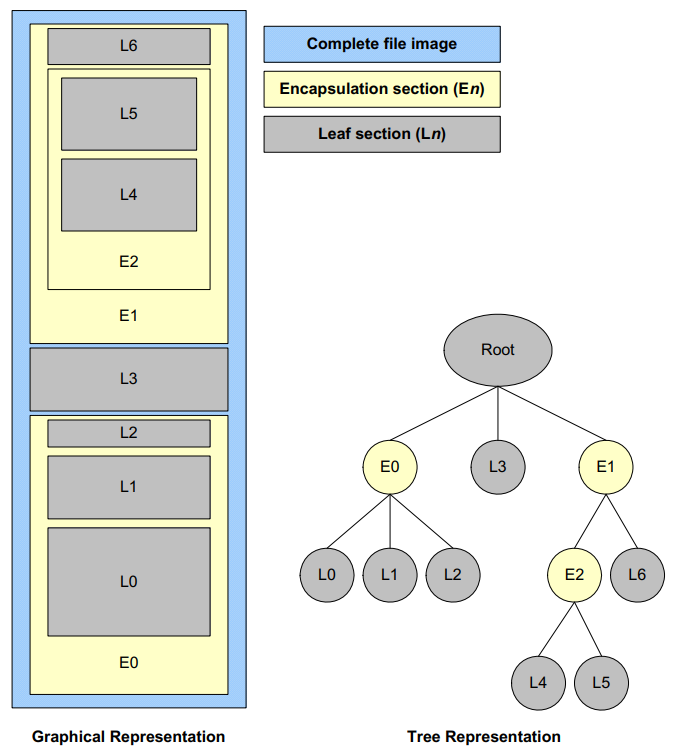
\includegraphics[width=0.9\linewidth]{architecture/firmware-file-system-representation}
	\caption{Example File System Image}\label{fig:architecture-firmware-file-system-representation}
\end{figure}

In the example shown in Figure \ref{fig:architecture-firmware-file-system-representation}, the file image root contains two encapsulation sections (E0 and E1) and one leaf section (L3). The first encapsulation section (E0) contains children, all of which are leaves (L0, L1, and L2). The second encapsulation section (E1) contains two children, one that is an encapsulation (E2) and the other that is a leaf (L6). The last encapsulation section (E2) has two children that are both leaves (L4 and L5).

In the PEI phase, section-related services are provided through the PEI Service Table, using \verb|FfsFindSectionData|. In the DXE phase, section-related services are provided through the \verb|EFI_FIRMWARE_VOLUME2_PROTOCOL| services attached to a volume's handle (\verb|ReadSection|).

\subsection{Firmware File Section Types}
Table \ref{table:architectural-section-types} list outs the defined architectural section types.

\begin{table}[!htbp]
	\centering
	\renewcommand{\arraystretch}{1.2}
	\caption{Architectural Section Types}\label{table:architectural-section-types}
	\begin{tabular}{p{7cm} | l | p{5cm}}
		Name & Value & Description
		\\ \hline \hline
		\verb|EFI_SECTION_COMPRESSION| & $ 0x1 $ & Encapsulation section where other sections are compressed
		\\ \hline
		\verb|EFI_SECTION_GUID_DEFINED| & $ 0x2 $ & Encapsulation section used during the build process but not required for execution
		\\ \hline
		\verb|EFI_SECTION_DISPOSABLE| & $ 0x3 $ & Encapsulation section used during the build process but not required for execution
		\\ \hline
		\verb|EFI_SECTION_PE32| & $ 0x10 $ & PE32+ Executable image
		\\ \hline
		\verb|EFI_SECTION_PIC| & $ 0x11 $ & Position-Independent Code
		\\ \hline
		\verb|EFI_SECTION_TE| & $ 0x12 $ & Terse Executable Image
		\\ \hline
		\verb|EFI_SECTION_DXE_DEPEX| & $ 0x13 $ & DXE Dependency Expression
		\\ \hline
		\verb|EFI_SECTION_VERSION| & $ 0x14 $ & Version, Text and numeric
		\\ \hline
		\verb|EFI_SECTION_USER_INTERFACE| & $ 0x15 $ & User-Friendly name of the driver
		\\ \hline
		\verb|EFI_SECTION_COMPATIBILITY16| & $ 0x16 $ & DOS-style 16-bit EXE
		\\ \hline
		\verb|EFI_SECTION_FIRMWARE_VOLUME_IMAGE| & $ 0x17 $ & PI Firmware Volume Image
		\\ \hline
		\verb|EFI_SECTION_FREEFORM_SUBTYPE_GUID| & $ 0x18 $ & Raw data with GUID in header to define format
		\\ \hline
		\verb|EFI_SECTION_RAW| & $ 0x19 $ & Raw data
		\\ \hline
		\verb|EFI_SECTION_PEI_DEPEX| & $ 0x1b $ & PEI Dependency Expression
		\\ \hline
		\verb|EFI_SECTION_SMM_DEPEX| & $ 0x1c $ & Leaf section type for determining the dispatch order for an MM Traditional driver in MM Traditional Mode or MM Standalone driver in MM Standalone Mode.
		\\ \hline
	\end{tabular}
\end{table}

\subsection{PI Architecture Firmware File System Format}
This section describes the standard binary encoding for PI Firmware Files, PI Firmware Volumes, and the PI Firmware File System. Implementations that allow the non-vendor firmware files or firmware volumes to be introduced into the system must support the standard formats. This section also describes how features of the standard format map into the standard PEI and DXE interfaces.

The standard firmware file and volume format also introduces additional attributes and capabilities that are used to guarantee the integrity of the firmware volume. The standard format is broken into three levels: the firmware volume format, the firmware file system format, and the firmware file format.

\begin{figure}[!htbp]
	\centering
	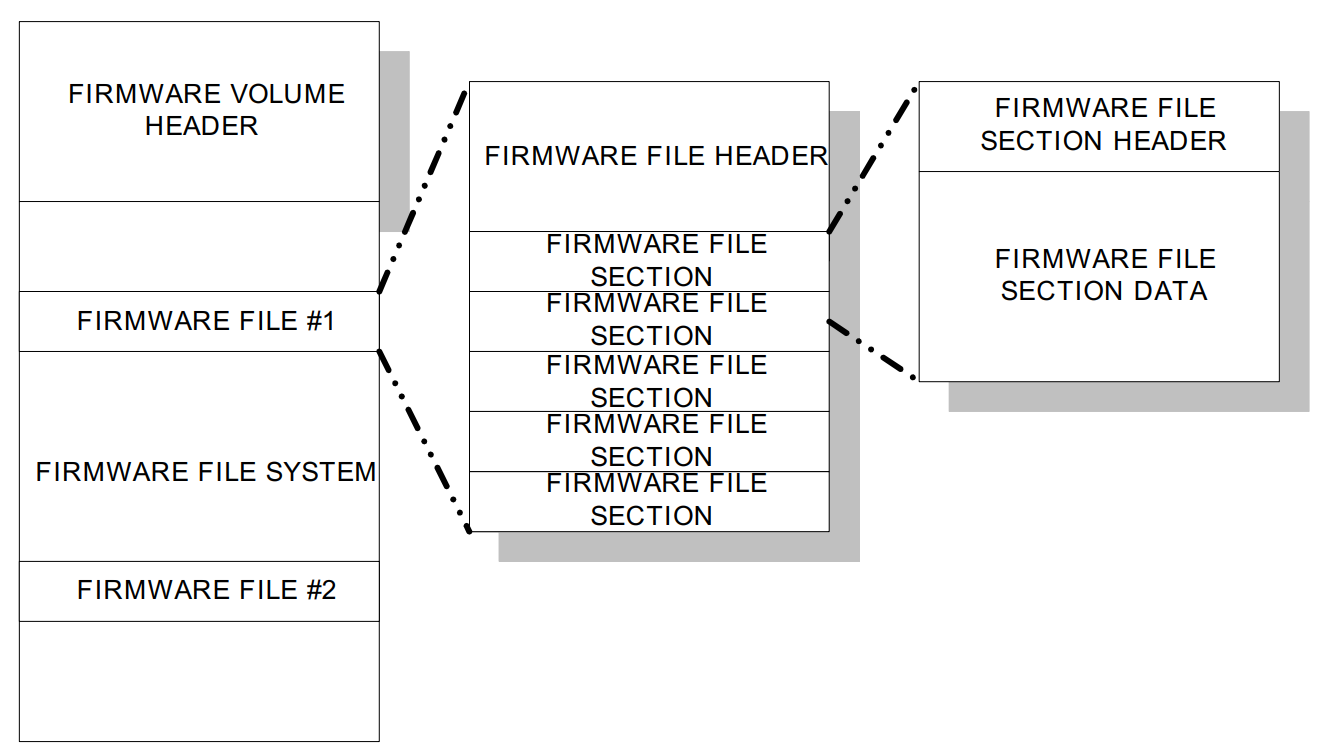
\includegraphics[width=0.8\linewidth]{architecture/the-firmware-volume-format}
	\caption{The Firmware Volume Format}\label{fig:architecture-the-firmware-volume-format}
\end{figure}

The standard firmware volume format (Figure \ref{fig:architecture-the-firmware-volume-format}) consists of two parts: the firmware volume header and the firmware volume data. The firmware volume header describes all of the attributes specified in “Firmware Volumes” on Table \ref{table:firmware-volume-attributes}. The header also contains a GUID which describes the format of the firmware file system used to organize the firmware volume data. The firmware volume header can support other firmware file systems other than the PI Firmware File System.

The PI Firmware File System format describes how firmware files and free space are organized
within the firmware volume.

The PI Firmware File format describes how files are organized. The firmware file format consists of
two parts: the firmware file header and the firmware file data.

\subsubsection{Firmware Volume Format}
he PI Architecture Firmware Volume format describes the binary layout of a firmware volume.
The firmware volume format consists of a header followed by the firmware volume data. The
firmware volume header is described by \verb|EFI_FIRMWARE_VOLUME_HEADER|.
The format of the firmware volume data is described by a GUID. Valid files system GUID values
are \verb|EFI_FIRMWARE_FILE_SYSTEM2_GUID| and \verb|EFI_FIRMWARE_FILE_SYSTEM3_GUID|.

\subsubsection{Firmware File System Format}
The PI Architecture Firmware File System is a binary layout of file storage within firmware
volumes. It is a flat file system in that there is no provision for any directory hierarchy; all files
reside in the root directly. Files are stored end to end without any directory entry to describe which files are present. Parsing the contents of a firmware volume to obtain a listing of files present requires walking the firmware volume from beginning to end.

\paragraph{Firmware File System GUID} The PI Architecture firmware volume header contains a data field for the file system GUID. There are two valid FFS file system, the GUID is defined as \verb|EFI_FIRMWARE_FILE_SYSTEM2_GUID| and \verb|EFI_FIRMWARE_FILE_SYSTEM3_GUID|.
If the FFS file system is backward compatible with \verb|EFI_FIRMWARE_FILE_SYSTEM2_GUID| and supports files larger than $ 16 \ MB $ then \verb|EFI_FIRMWARE_FILE_SYSTEM3_GUID| is used.

\paragraph{Volume Top File} A Volume Top File (VTF) is a file that must be located such that the last byte of the file is also the last byte of the firmware volume. Regardless of the file type, a VTF must have the file name GUID of \verb|EFI_FFS_VOLUME_TOP_FILE_GUID|.
Firmware file system driver code must be aware of this GUID and insert a pad file as necessary to guarantee the VTF is located correctly at the top of the firmware volume on write and update operations. File length and alignment requirements must be consistent with the top of volume. Otherwise, a write error occurs and the firmware volume is not modified.

\subsection{Firmware File Format (\gls{ffs})}
All FFS files begin with a header that is aligned on an $ 8-byte $ boundary with respect to the beginning
of the firmware volume. FFS files can contain the following parts:
\begin{itemize}
	\item Header
	\item Data
\end{itemize}

It is possible to create a file that has only a header and no data, which consumes 24 bytes of space.
This type of file is known as a zero-length file.

If the file contains data, the data immediately follows the header. The format of the data within a file
is defined by the Type field in the header, either \verb|EFI_FFS_FILE_HEADER| or \verb|EFI_FFS_FILE_HEADER2|.

Figure \ref{fig:architecture-typical-ffs-file-layout-less-than-16MB} illustrates the layout of a (typical i.e. \verb|EFI_FFS_FILE_HEADER|) PI Architecture Firmware File smaller than $ 16 Mb $.

\begin{figure}[!htbp]
	\centering
	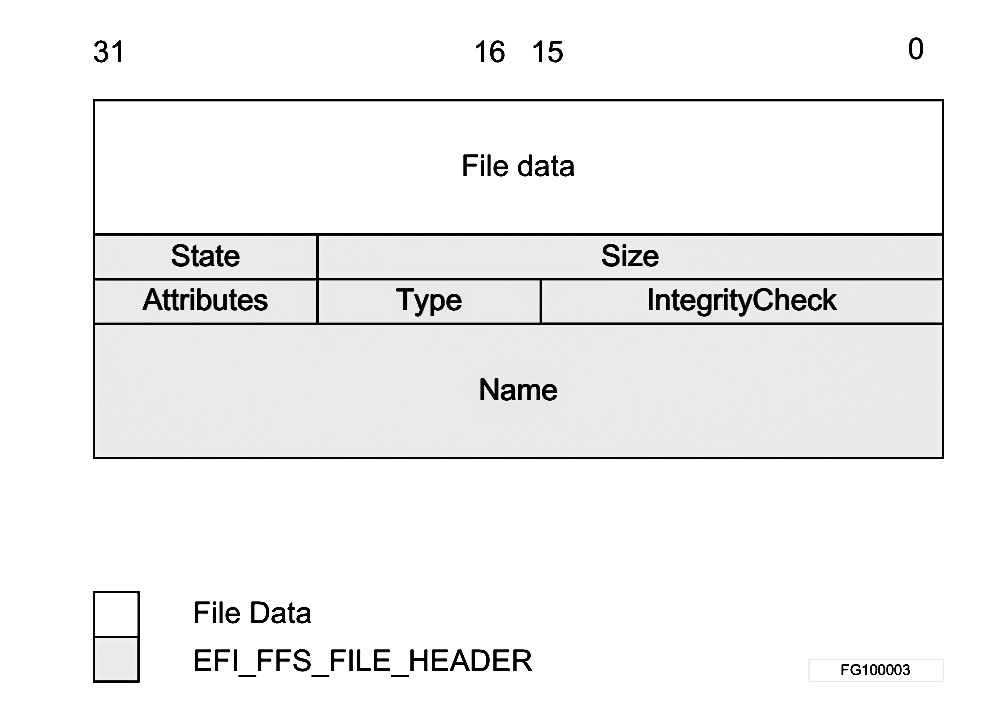
\includegraphics[width=0.8\linewidth]{architecture/typical-ffs-file-layout-less-than-16MB}
	\caption{Typical FFS File Layout}\label{fig:architecture-typical-ffs-file-layout-less-than-16MB}
\end{figure}

Figure \ref{fig:architecture-typical-ffs-file-layout-greater-than-16MB} illustrates the layout of a PI Architecture Firmware File larger than $ 16 Mb $.

\begin{figure}[!htbp]
	\centering
	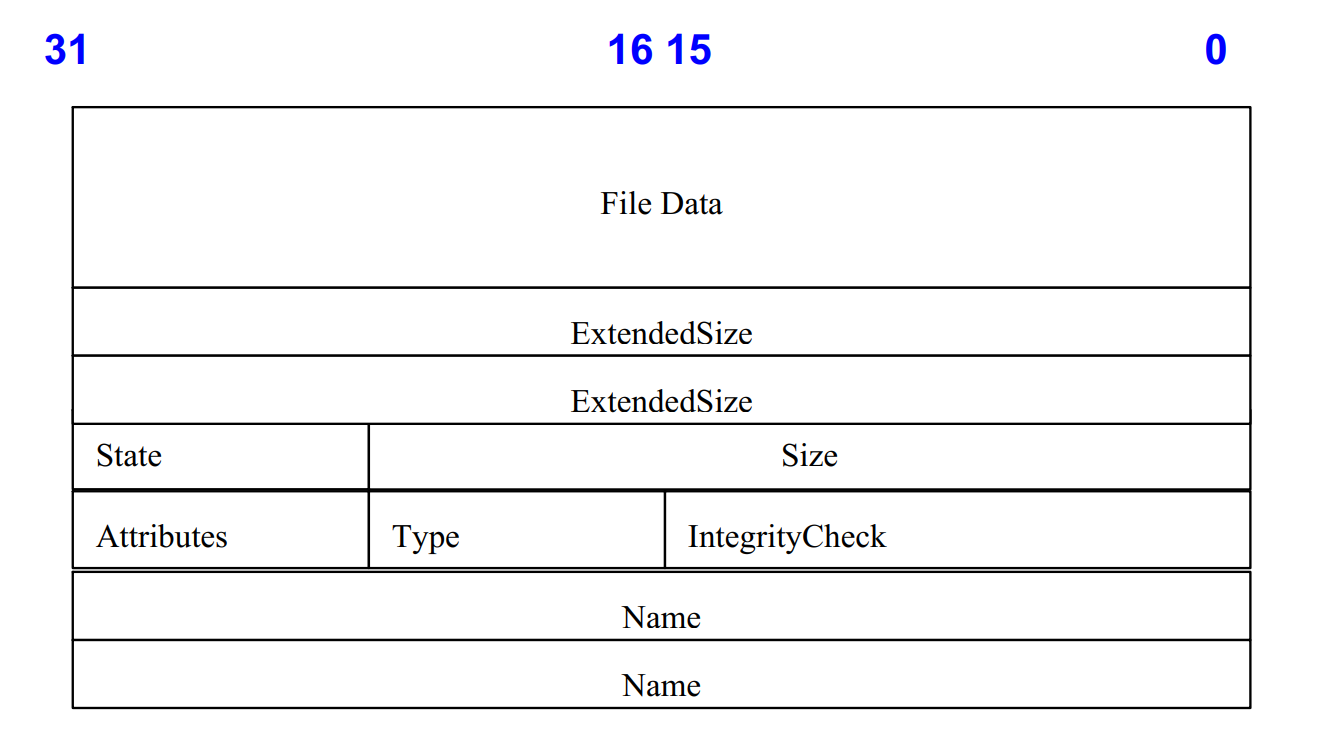
\includegraphics[width=0.8\linewidth]{architecture/typical-ffs-file-layout-greater-than-16MB}
	\caption{File Header 2 layout for files larger than $ 16Mb $}\label{fig:architecture-typical-ffs-file-layout-greater-than-16MB}
\end{figure}


\subsection{Firmware File Section Format}
This section describes the standard firmware file section layout.
Each section begins with a section header, followed by data defined by the section type.
The section headers aligned on 4 byte boundaries relative to the start of the file's image. If padding is
required between the end of one section and the beginning of the next to achieve the 4-byte
alignment requirement, all padding bytes must be initialized to zero.
Many section types are variable in length and are more accurately described as data streams rather
than data structures.

Regardless of section type, all section headers begin with a $ 24-bit $ integer indicating the section size,
followed by an 8-bit section type. The format of the remainder of the section header and the section
data is defined by the section type. If the section size is $ 0xFFFFFF $ then the size is defined by a $ 32-
bit $ integer that follows the $ 32-bit $ section header. Figures \ref{fig:architecture-format-of-a-section-below-16Mb} and \ref{fig:architecture-format-of-a-section-above-16Mb} shows the general format of a section.

\begin{figure}[!htbp]
	\centering
	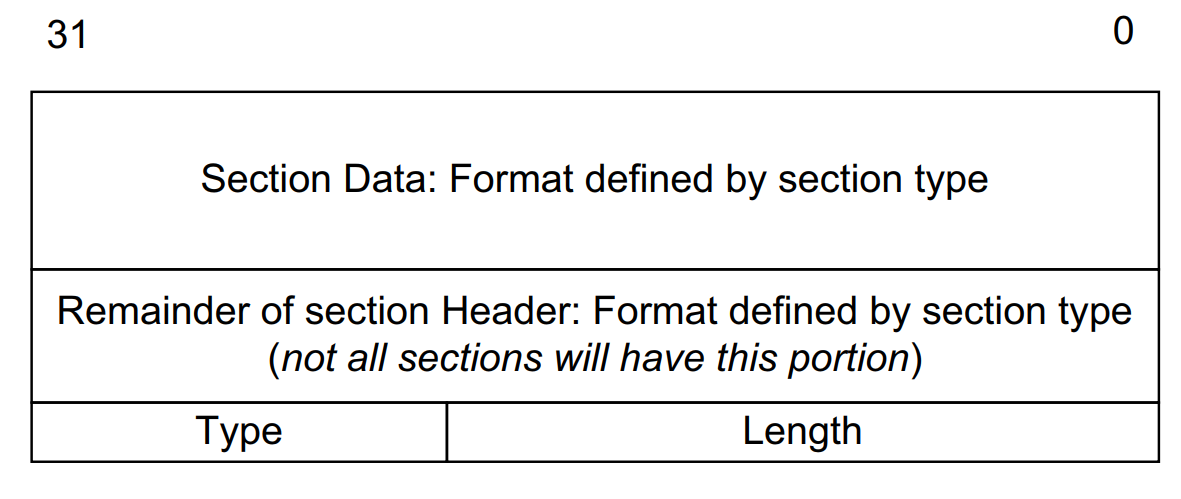
\includegraphics[width=0.8\linewidth]{architecture/format-of-a-section-below-16Mb}
	\caption{Format of a Section below $ 16Mb $}\label{fig:architecture-format-of-a-section-below-16Mb}
\end{figure}

\begin{figure}[!htbp]
	\centering
	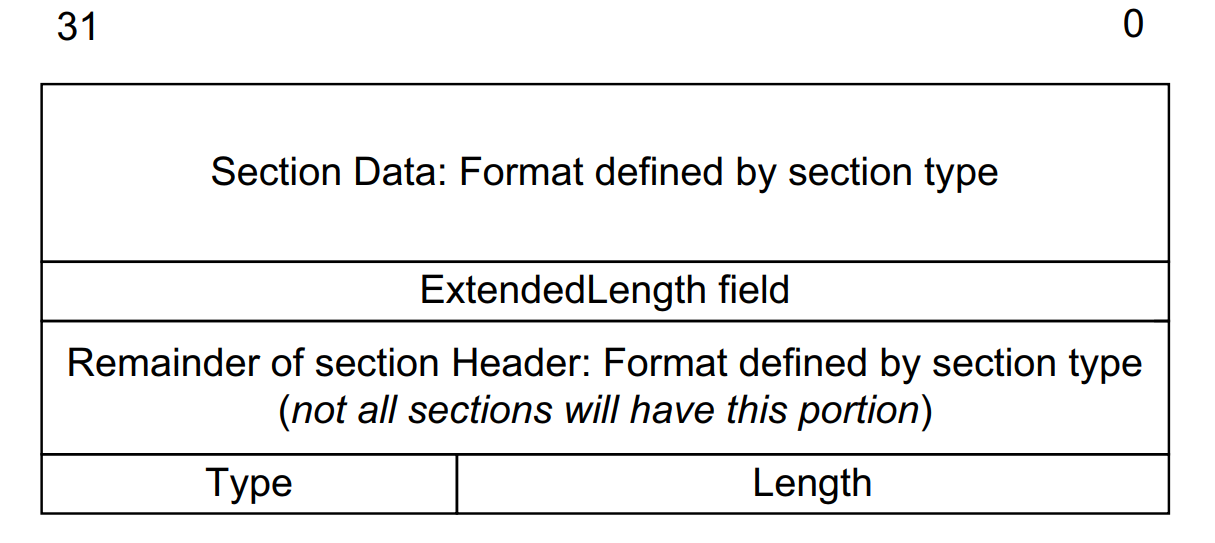
\includegraphics[width=0.8\linewidth]{architecture/format-of-a-section-above-16Mb}
	\caption{Format of a Section using ExtendedLegth field $ 16Mb $}\label{fig:architecture-format-of-a-section-above-16Mb}
\end{figure}


\subsection{File System Initialization}\label{subsection:file-system-initialization}
The algorithm \ref{code:architecture-file-system-initialization} describes a method of FFS initialization that ensures FFS file corruption can be detected regardless of the cause.

The State byte of each file must be correctly managed to ensure the integrity of the file system is
not compromised in the event of a power failure during any FFS operation. It is expected that an FFS
driver will produce an instance of the Firmware Volume Protocol and that all normal file operations
will take place in that context. All file operations must follow all the creation, update, and deletion
rules described in this specification to avoid file system corruption.

The following \verb|FvCheck()| pseudo code must be executed during FFS initialization to avoid file
system corruption. If at any point a failure condition is reached, then the firmware volume is
corrupted and a crisis recovery is initiated.All FFS files, including files of type
\verb|EFI_FV_FILETYPE_FFS_PAD| must be evaluated during file system initialization. It is legal for
multiple pad files with this file type to have the same Name field in the file header. No checks for
duplicate files should be performed on pad files.

\inputminted{c}{code/architecture-file-system-initialization.c}\label{code:architecture-file-system-initialization}

\subsection{Traversal and Access to Files}
The Security (SEC), PEI, and early DXE code must be able to traverse the FFS and read and execute
files before a write-enabled DXE FFS driver is initialized. Because the FFS may have
inconsistencies due to a previous power failure or other system failure, it is necessary to follow a set
of rules to verify the validity of files prior to using them. It is not incumbent on SEC, PEI, or the
early read-only DXE FFS services to make any attempt to recover or modify the file system. If any
situation exists where execution cannot continue due to file system inconsistencies, a recovery boot
is initiated.

There is one inconsistency that the SEC, PEI, and early DXE code can deal with without initiating a
recovery boot. This condition is created by a power failure or other system failure that occurs during
a file update on a previous boot. Such a failure will cause two files with the same file name GUID to
exist within the firmware volume. One of them will have the \verb|EFI_FILE_MARKED_FOR_UPDATE|
bit set in its State field but will be otherwise a completely valid file. The other one may be in any
state of construction up to and including \verb|EFI_FILE_DATA_VALID|. All files used prior to the
initialization of the write-enabled DXE FFS driver must be screened with this test prior to their use.
If this condition is discovered, it is permissible to initiate a recovery boot and allow the recovery
DXE to complete the update.
The following pseudo code describes the method for determining which of these two files to use.
The inconsistency is corrected during the write-enabled initialization of the DXE FFS driver.

\inputminted{c}{code/architecture-traversal-and-file-access.c}\label{code:architecture-traversal-and-file-access}


\paragraph{Note} There is no check for duplicate files once a file in the \verb|EFI_FILE_DATA_VALID| state is located.
The condition where two files in a single firmware volume have the same file name GUID and are
both in the \verb|EFI_FILE_DATA_VALID| state cannot occur if the creation and update rules that are
defined in this specification are followed.

\subsection{File Integrity and State}
File corruption, regardless of the cause, must be detectable so that appropriate file system repair
steps may be taken. File corruption can come from several sources but generally falls into three
categories:
\begin{itemize}
	\item General failure
	\item Erase failure
	\item Write failure
\end{itemize}

A general failure is defined to be apparently random corruption of the storage media. This
corruption can be caused by storage media design problems or storage media degradation, for
example. This type of failure can be as subtle as changing a single bit within the contents of a file.
With good system design and reliable storage media, general failures should not happen. Even so,
the FFS enables detection of this type of failure.

An erase failure occurs when a block erase of firmware volume media is not completed due to a
power failure or other system failure. While the erase operation is not defined, it is expected that
most implementations of FFS that allow file write and delete operations will also implement a
mechanism to reclaim deleted files and coalesce free space. If this operation is not completed
correctly, the file system can be left in an inconsistent state.
Similarly, a write failure occurs when a file system write is in progress and is not completed due to a
power failure or other system failure. This type of failure can leave the file system in an inconsistent
state.

All of these failures are detectable during FFS initialization, and, depending on the nature of the
failure, many recovery strategies are possible. Careful sequencing of the State bits during normal
file transitions is sufficient to enable subsequent detection of write failures. However, the State
bits alone are not sufficient to detect all occurrences of general and/or erase failures. These types of
failures require additional support, which is enabled with the file header \verb|IntegrityCheck| field.
For sample code that provides a method of FFS initialization that can detect FFS file corruption,
regardless of the cause, see “File System Initialization” on Section \ref{subsection:file-system-initialization}.



